\documentclass[
	paper=a4,
	fontsize=10pt,
	nenglish
]{scrartcl}

% Basics
% ===========================================================
\usepackage[english]{babel}
\usepackage[T1]{fontenc}
\usepackage{csquotes}
\usepackage{etex}
\usepackage{xcolor}
\usepackage{xspace}
\usepackage{etoolbox}
\usepackage{xparse}
\usepackage{ifthen}
\usepackage{calc}
% ===========================================================

% graphics, documents, links
% ===========================================================
\usepackage{graphicx}
\usepackage{graphics}
\usepackage{svg}
\usepackage{pdfpages}
\usepackage{hyperref}
\usepackage{epstopdf}
\AppendGraphicsExtensions{.pdf}


% ===========================================================
% Figures
% ===========================================================
\usepackage{float}
\NewDocumentCommand{\Fig}{ O{1} O{H} m m m }{%
	\begin{figure}[#2]
		\centering
		\includegraphics[width=#1\linewidth]{#3}%
		\caption{#4}%
		\label{fig:#5}%
	\end{figure}%
}



% Fonts & Typography
% ===========================================================
\linespread{1.25}
\usepackage{sourcecodepro}
\usepackage[default]{sourcesanspro}
\usepackage{amsfonts}
\usepackage{stmaryrd}
\usepackage{bbm}
\usepackage{bm}
\newcommand{\code}[1]{\texttt{#1}}
\usepackage{xspace}
\makeatletter 
\xspaceaddexceptions{\grqq \grq \csq@qclose@i \} } 
\makeatother
\usepackage{multicol}
\usepackage{vwcol}
\usepackage{soul}
\usepackage{eurosym}
% ===========================================================


% Mathe-Pakete
% ===========================================================
\usepackage{mathtools}
\usepackage{amssymb}
\usepackage[bigdelims]{newtxmath}
\usepackage{wasysym}
% ===========================================================

% TikZ -- hope we dont need it
% ===========================================================
%\usepackage{tikz}
%\usepackage{tikz-cd}          
%\usetikzlibrary{arrows.meta}    
%\usetikzlibrary{shadows}
%\usetikzlibrary{calc}
%\usetikzlibrary{backgrounds}  
%\usetikzlibrary{patterns}
%\tikzset{>=Latex}

%\usepackage{tikz-qtree}
%\usetikzlibrary{positioning, shapes.geometric}
% ===========================================================

% pgfplots - dont needed
% ===========================================================
% \usepackage{pgfplots}
% \pgfplotsset{width=10cm,compat=1.9}
% ===========================================================

% Tabel
% ===========================================================
\usepackage{tabularray} % best tables
% ===========================================================

% listings
% ===========================================================
\usepackage{listingsutf8}
\usepackage[most]{tcolorbox}
% \begin{lstlisting}[style=pseudo]
\lstdefinestyle{pseudo}{
	belowcaptionskip=1\baselineskip,
	breaklines=true,
	showstringspaces=false,
	keepspaces,
	showstringspaces=false,
	basicstyle=\small,
	keywordstyle=\bfseries,
	commentstyle=\itshape\color{gray},
	numbers=left,
	numberstyle=\tiny\ttfamily\color{darkgray},
	inputencoding=utf8/latin1,
	tabsize=2,
	mathescape,
	morekeywords={if, then, return, end, function, for, to, do, while, else, and, procedure},
	literate={:=}{$\leftarrow$}1,
	moredelim=[is][\normalfont\raggedleft]{|}{|}
}

% really complex stuff for nice python code snippets
\newlength{\LstNumField}
\setlength{\LstNumField}{40em}
\makeatletter
\renewcommand{\thelstnumber}{\ifnum\value{lstnumber}<10 0\fi\arabic{lstnumber}}
\makeatother
\makeatletter
\newcommand{\zebra}[2]{%
	\begingroup
	\lst@basicstyle
	\ifodd\value{lstnumber}%
	\color{#1}%
	\else
	\color{#2}%
	\fi
	\rlap{\hspace*{\lst@numbersep}%
		\color@block{1.015\linewidth}{\ht\strutbox}{\dp\strutbox}%
	}	
	\endgroup 	
}
\makeatother

\lstdefinestyle{python}{
	language=Python,
	%belowcaptionskip=1\baselineskip,
	breaklines=false,
	showstringspaces=false,
	keepspaces,
	basicstyle=\small\ttfamily,
	keywordstyle=\bfseries\color{blue},
	commentstyle=\itshape\color{green},
	stringstyle=\color{orange},
	numbers=left,
	inputencoding=utf8,
	tabsize=2,
	numberstyle=\ttfamily\zebra{gray!15}{gray!2},
	numbersep=2.2em}

\DeclareRobustCommand{\PythonFile}[3]{
	\begin{tcolorbox}[colback=gray!15, colframe=black, boxrule=0.5pt, arc=1pt, left=16.5pt, right=-9.5pt, top=-5pt, bottom=-5pt,boxsep=0pt]
			\lstinputlisting[
			style=python,
			firstline=#2,
			lastline=#3,
			firstnumber=#2
			]{#1}
		\end{tcolorbox}
		\vspace{-4pt}
		{\tiny #1: Line #2-#3 \medskip\par}
}
% ===========================================================

% Bibliography for References
% ===========================================================
  \usepackage[
	  backend=biber,
	  style=numeric,
	  sorting=ynt,
	  citestyle=numeric
  ]{biblatex}
  \addbibresource{./modules/references.bib}
  \renewcommand*{\mkbibbrackets}[1]{\textsuperscript{[#1]}}
  \nocite{*}    

% Hyperlinks within Document and urls
\hypersetup{
	colorlinks=true,
	linkcolor=black,
	filecolor=magenta,      
	urlcolor=cyan,
	pdfpagemode=FullScreen,
	citecolor=blue
}
\urlstyle{same}

% ===========================================================



% table of contents
% ===========================================================
\newcommand{\toc}{
		\tableofcontents
		\pagebreak
}
% ===========================================================

% Empty Line
% ===========================================================
\newcommand{\blank}{\phantom{ }\\}
% ===========================================================


% Quotes
% ===========================================================
\newcommand{\qt}[1]{\glqq #1\grqq \xspace }
% ===========================================================

% Shortcuts
% ===========================================================
\newcommand{\B}{\mathbb{B}}
\newcommand{\C}{\mathbb{C}}
\newcommand{\N}{\mathbb{N}}
\newcommand{\Q}{\mathbb{Q}}
\newcommand{\R}{\mathbb{R}}
\newcommand{\Z}{\mathbb{Z}}
\newcommand{\oh}{\mathcal{O}}

\newcommand{\ra}{\rightarrow}
\newcommand{\imp}{\Rightarrow}
\newcommand{\limp}{\Leftarrow}
\newcommand{\eq}{\Leftrightarrow}


\newcommand{\ol}[1]{\overline{#1}}
\newcommand{\wt}[1]{\widetilde{#1}}
\newcommand{\wh}[1]{\widehat{#1}}

\DeclareMathOperator{\id}{id}         % Identity
\DeclareMathOperator{\pot}{\mathcal{P}}    % Potency Set
% ===========================================================

% Brackets
% ===========================================================
\DeclarePairedDelimiter{\absolut}{\lvert}{\rvert}    % Abs
\DeclarePairedDelimiter{\ceiling}{\lceil}{\rceil}    % Ceil
\DeclarePairedDelimiter{\Floor}{\lfloor}{\rfloor}    % Floor
\DeclarePairedDelimiter{\Norm}{\lVert}{\rVert}      % Norm
\DeclarePairedDelimiter{\sprod}{\langle}{\rangle}    
\DeclarePairedDelimiter{\enbrace}{(}{)}          % n
\DeclarePairedDelimiter{\benbrace}{\lbrack}{\rbrack}  
\DeclarePairedDelimiter{\penbrace}{\{}{\}}        
\newcommand{\Underbrace}[2]{{\underbrace{#1}_{#2}}}   

\newcommand{\abs}[1]{\absolut*{#1}}
\newcommand{\ceil}[1]{\ceiling*{#1}}
\newcommand{\flo}[1]{\Floor*{#1}}
\newcommand{\no}[1]{\Norm*{#1}}
\newcommand{\sk}[1]{\sprod*{#1}}
\newcommand{\enb}[1]{\enbrace*{#1}}
\newcommand{\penb}[1]{\penbrace*{#1}}
\newcommand{\benb}[1]{\benbrace*{#1}}

\makeatletter
\renewcommand*\env@matrix[1][*\c@MaxMatrixCols c]{%
	\hskip -\arraycolsep
	\let\@ifnextchar\new@ifnextchar
	\array{#1}}
\makeatother
% ===========================================================

\date{\today}

% use \PythonFile{<<path>>}{<<firstline>>}{<<lastline>>} to include a code snipped

% use \begin{tblr} \end{tblr} for tables

% further information about references: https://www.overleaf.com/learn/latex/Bibliography_management_with_biblatex
%  short version: use \cite{} in the text and add an entry of your source to the references.bib

% Let's use an own file per Section

% for Images and diagrams use
%	\figure[width([0,1])]{<<path>>}{<<caption>>}{<<label>>} % Label starts with fig:
%	only add a name without special characters or spaces. You dont have to write a
%	width. standard is 1. Example: 
%		\Fig[0.5]{./assets/universityLogo.png}{very nice Logo}{logo}

\begin{document}
\title{Projecttitle}
\date{\today}


\begin{titlepage}
	\centering
	\includegraphics[width=0.5\textwidth]{./assets/universityLogo}\par\vspace{1cm}
	
	\vspace{1cm}
	{\huge\bfseries <<Project title>> \par}
	\vspace{1cm}
	{\Large\itshape Authors: Lorenz Kruse, Harshal Ghadge,Takkyon Kesselring, Luis Gebhardt, Luca Steinhausen, Martin Bruckmeier \par}
	\vspace{1cm}
	{\Large\itshape Supervisors: Jostein\par}
	\vspace{1cm}
	{\Large\bfseries Project report for DAT-215 ICT-Project in Autumn 2025\par}
	{\Large\normalfont \today \par}
	
	\vfill
	
	
	
	
\end{titlepage}
\paragraph{Preface}

This report is submitted as part of the course \textit{DAT215-G 25H Multimedieprosjekt} at the University of Agder. It documents the development and completion of our project \textbf{CircuitQuest -- A Logic Gate Educational Tool}, created with the objective of providing an engaging and accessible learning environment for understanding digital logic from fundamentals to advanced topics.

The project was carried out by the following group members: 
Martin Gregor Bruckmeier, Harshal Ghadge, Luis Antonio Gebhardt, 
Luca Alexander Detlef Steinhausen, Lorenz Kruse, and Tækkyon Ari Kesselring.

We would like to express our sincere gratitude to our project supervisor, \textbf{Jostein Nordengen}, for his continuous support, valuable guidance, and constructive feedback throughout the entire project process. His insights were instrumental in shaping the final outcome of CircuitQuest.

We also extend our appreciation to the course organiser, \textbf{Morgan Konnestad}, for his organisational efforts. In particular, we thank him for enabling the formation of an unusually large project group, which provided a valuable collaborative learning experience.

The work presented in this report is the result of our collective effort during the semester, and we hope it will serve as a useful contribution within the field of multimedia-based educational tools.

\vspace{1cm}
Grimstad, \today \\
On behalf of the project group


\pagebreak
\toc
% - Background
% - Problem definition
% - Assumptions and limitations
% - Literature study
% - 


\section{Introduction}
%TODO introduction

\subsection{Problem Definitioncumcumcum}
\section{Theoretical Background}
\label{sec:theoretical_background}

This project aims to gamify the understanding of computer architecture. To comprehend the educational scope of the application, it is necessary to understand the underlying principles of digital system design, ranging from elementary logic gates to the organization of a microprocessor. This section outlines the fundamental concepts of digital logic, sequential circuits, and the MIPS architecture upon which the application is based.

\subsection{Digital Logic and Combinational Circuits}
Digital computers operate on binary data, representing information as sequences of zeros and ones (low and high voltage levels). The fundamental building blocks of these systems are \textit{logic gates}, which implement Boolean algebraic functions. The most basic gates include AND, OR, and NOT. By combining these primitives, functionally complete sets can be formed, allowing for the construction of any complex logical operation.

Circuits constructed from these gates without any memory elements are known as \textit{Combinational Circuits}. In these circuits, the output is a pure function of the present inputs. The application simulates several key combinational components used in processor design:
\begin{itemize}
    \item \textbf{Multiplexers (MUX):} Components that select one input signal from multiple sources based on a control signal.
    \item \textbf{Decoders:} Circuits that convert an $n$-bit input code into one of $2^n$ output lines, essential for interpreting operation codes.
    \item \textbf{Arithmetic Logic Unit (ALU):} The computational core of the processor, capable of performing arithmetic (ADD, SUB) and logical (AND, OR) operations.
\end{itemize}

\subsection{Sequential Circuits and State}
While combinational circuits handle data manipulation, computation requires the storage of intermediate results. \textit{Sequential Circuits} differ from combinational logic in that their output depends not only on the current inputs but also on the past history of inputs, effectively possessing a "state."

The basic storage element is the \textit{Latch} or \textit{Flip-Flop}, typically constructed from cross-coupled gates (e.g., NAND or NOR). These elements can store a single bit of information. In a synchronous processor design, these state elements are updated on the edge of a global clock signal. By grouping multiple flip-flops, we create \textbf{Registers}, which form the high-speed memory (Register File) of the processor.

\subsection{MIPS Architecture}
The final educational goal of the application is the construction of a MIPS (Microprocessor without Interlocked Pipeline Stages) processor. MIPS is a Reduced Instruction Set Computer (RISC) architecture, characterized by a small set of simple, regular instructions. The design focuses on a \textit{Single-Cycle Datapath}, where every instruction takes exactly one clock cycle to complete.

The architecture distinguishes between the \textbf{Datapath} and the \textbf{Control Unit}:
\begin{itemize}
    \item \textbf{The Datapath} consists of the functional units (ALU, Registers, Memory) and the interconnections (buses) that process data. It executes the "Fetch-Decode-Execute" cycle: retrieving an instruction from Instruction Memory, decoding its fields to read registers, performing the operation in the ALU, and optionally accessing Data Memory or writing back to the Register File.
    \item \textbf{The Control Unit} acts as the brain of the processor. Based on the 6-bit opcode (and occasionally the "funct" field) of the instruction, it generates the necessary control signals (e.g., \textit{RegDst}, \textit{ALUSrc}, \textit{MemWrite}) to steer data through the multiplexers and activate the correct units in the datapath.
\end{itemize}

\begin{figure}[htbp]
    \centering
    \includegraphics[width=0.9\linewidth]{assets/mips-cpu.pdf}
    \caption{Single-cycle MIPS datapath adapted from \cite{referenceBookEnglish}.\\\textbf{Note.} The example processor in level 21 is for demonstration purposes and does not implement jump functionality.}
    \label{fig:mips_single_cycle}
\end{figure}

In a single-cycle implementation, the clock cycle must be long enough to accommodate the slowest instruction (typically a Load Word instruction), rendering it less efficient than pipelined designs but significantly easier to model and understand for educational purposes.
% - How to install
% - How to use everything, Teaching Mode and Sandboxmode
% - Levelprogression, recommend Levels
% - Usage as Customcomponents


\section{Program Usage}
\subsection{Installation and Executing From Source}
% Im going to write this section as the project stands currently, I.E. using a venv

Running the program should be done from a terminal.

\begin{itemize}
    \item For Windows: Use powershell, cd to the project root directory
    \item For Linux: In your preferred terminal, cd to the project root directory
    \item For Mac: Ask Lorenz\\
\end{itemize}

\paragraph{Instructions}

Dependencies:
\begin{itemize}
    \item \texttt{python}, Version 3.13 was used in development, but newer versions will likely work.\\

\end{itemize}

Step 1, setting up the environment:
\begin{itemize}
    \item All: \texttt{python3.13 -m venv env}\\

\end{itemize}

Step 2, entering the environment:
\begin{itemize}
    \item Linux: \texttt{source env/bin/activate}
    \item Windows: \texttt{\& "./env/Scripts/Activate.ps1"}.  If an error comes up saying that running scripts is disabled, 
    run \texttt{Set-ExecutionPolicy -ExecutionPolicy Unrestricted -Scope Process} first.
    \item Mac: \\

\end{itemize}

Step 3, installing/updating packages:
\begin{itemize}
    \item All: \texttt{pip install -r requirements.txt}.\\

\end{itemize}

Step 4, Running:
\begin{itemize}
    \item All: \texttt{python3 -m src.main}.\\

\end{itemize}

\section{Group Management and Methodology}
\label{sec:group_management}

Managing a group of six students presents different challenges compared to the smaller teams typically found in this course. To prevent the project from becoming chaotic, we needed a clear way to organize our work and communication. However, rather than strictly following a complex management framework, we chose a pragmatic approach that adapted Agile principles to our specific needs.

\subsection{Team Structure and Responsibilities}
We decided against assigning formal leadership roles such as a Project Manager. Instead, we operated with a flat hierarchy where every member had equal say in decision-making. To work efficiently, we naturally divided into two main areas of focus based on the application's architecture:

\begin{itemize}
    \item \textbf{Backend:} Luis, Tækkyon, and Martin focused on the core logic, including the gate implementation and processor simulation.
    \item \textbf{Frontend:} Luca, Lorenz, and Harshal focused on the Graphical User Interface (GUI) and user interactions.
\end{itemize}

This separation was not strict; members often helped out in the other domain when bottlenecks appeared. This flexibility allowed us to utilize the full capacity of the team without being limited by rigid role definitions.

\subsection{Workflow and Communication}
Our workflow was organized in weekly cycles. We held one synchronous meeting per week which served as our main synchronization point. During these sessions, we discussed the tasks completed in the previous week, identified any technical problems, and brought up new ideas. Once the status was clear, we defined the tasks for the upcoming week and distributed them among the team.

We used GitHub as our sole project management tool. By utilizing GitHub Issues and Projects, we kept our planning close to the code, which reduced the complexity of using external tools.

\subsection{Quality Control and Reflection}
To ensure the stability of our code, we established a "Quality Gate" system using GitHub Actions. Theoretically, our protocol required that every change be submitted via a Pull Request and reviewed by another member before being merged into the \textit{main} branch.

In the early and middle stages of the project, this discipline was maintained and helped us catch several errors. However, as the final deadline approached and the pressure to deliver features increased, we became less strict with this rule. Towards the end, code was occasionally merged with little to no review to save time. In hindsight, this was a risky deviation from our workflow. While it allowed us to move faster in the short term, it potentially introduced instability that could have been avoided with better time management.

\subsection{Conflict Resolution}
Despite the large group size, we encountered very few interpersonal conflicts. Disagreements were almost exclusively technical. We resolved these by trusting the expertise of the person most involved in that specific part of the code. We believe the project ran smoothly largely because four of the members (Lorenz, Luis, Luca, and Martin) had previous experience working on software projects of this scale. This experience helped the group anticipate coordination issues before they became major problems.
\section{Program Structure}

The application architecture follows the \textbf{Model-View-Controller (MVC)} design pattern, which was selected to ensure a clear separation of concerns between the simulation logic, the user interface, and the application flow control. This separation facilitates modular development and testing, allowing the backend logic to evolve independently of the frontend visualization.

The source code is organized into four primary packages within the \texttt{src} directory, each responsible for a distinct layer of the application:

\begin{itemize}
    \item \textbf{Model (\texttt{src.model}):} This package encapsulates the core logic of the circuit simulator. It defines the abstract base class \texttt{LogicComponent} and its concrete implementations (e.g., logic gates, adders, and memory units). The model is responsible for the state of the simulation but contains no reference to the user interface.
    \item \textbf{View (\texttt{src.view}):} This package manages the graphical user interface (GUI) using the \texttt{PySide6} framework. It includes the main application window, scene definitions (e.g., \texttt{LevelScene}, \texttt{SandboxModeScene}), and the interactive grid.
    \item \textbf{Controller (\texttt{src.control}):} The controller layer acts as the intermediary between the model and the view. It orchestrates the application lifecycle, manages the loading of levels via the \texttt{LevelFileController}, and handles user interactions by updating the model accordingly.
    \item \textbf{Infrastructure (\texttt{src.infrastructure}):} This package contains shared utilities, most notably the \texttt{EventBus}.
\end{itemize}

The high-level dependencies and relationships between these packages are illustrated in Figure \ref{fig:package_diagram}.

\begin{figure}[H]
    \centering
    \includegraphics[width=0.8\textwidth]{./assets/package_Diagramm.pdf}
    \caption{Package diagram illustrating the dependencies between the application modules.}
    \label{fig:package_diagram}
\end{figure}
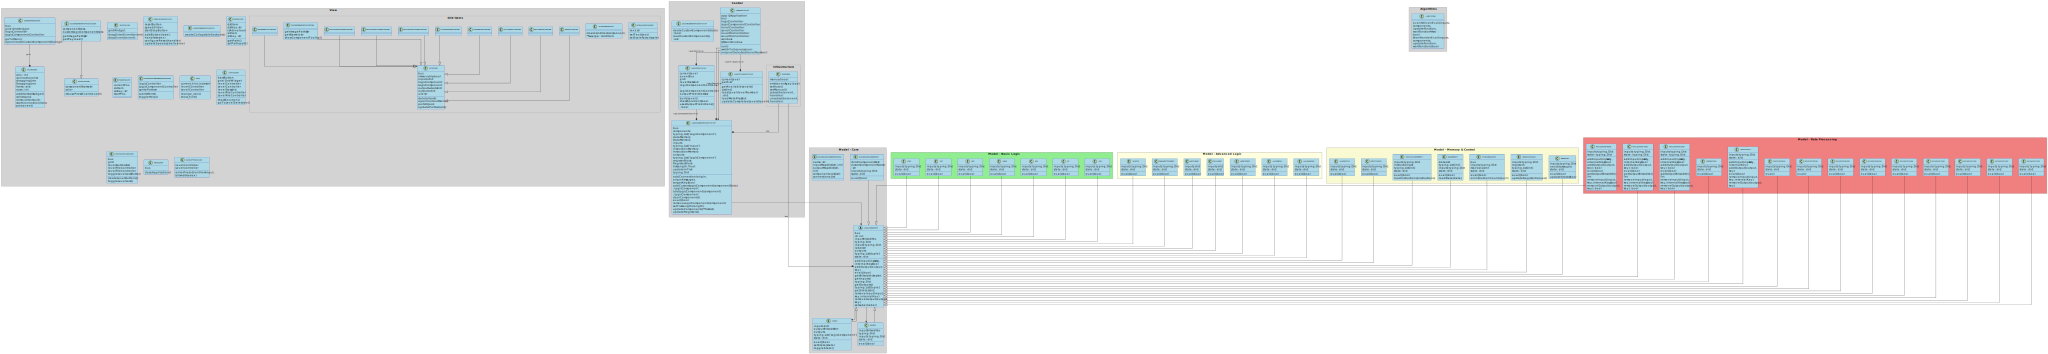
\includepdf[pages=-,fitpaper=true,angle=90]{./assets/classes_ICT-Project}
\subsection{Design Patterns and Architectural Decisions}

To maintain loose coupling between components, the project employs the \textbf{Event Bus} pattern. This is will further be explained in 6.2. Event bus and MVC decoupling.

Additionally, the \textbf{Factory Method} pattern is utilized within the view layer to manage the creation of grid items. The \texttt{GridItemFactory} class provides a static interface for instantiating the appropriate graphical representation (e.g., \texttt{InputGridItem}, \texttt{ALUAdvancedGridItem}) based on the type of \texttt{LogicComponent} provided. This abstraction isolates the \texttt{GridWidget} from the complexity of instantiating specific component subclasses, thereby adhering to the Open/Closed Principle regarding the addition of new component types.

The entry point of the application, \texttt{AppController}, initializes the main window and navigates between the distinct application states (Sandbox, Level Selection, and Level Interaction) by swapping the central widget of the main window, effectively functioning as a high-level state manager.   
% - Eventbus
% - Algorithms
% - CustonComponents



\section{Backend - interesting stuff}
% Frontend subsections
% Devide into scenes and components
% Gridwidget
% svg's
%


\section{Frontend Implementation}

The frontend of the application is designed to provide an interactive and responsive environment where students can visualize and manipulate logic circuits. This section details the technology stack, the architecture of the user interface, and the custom implementation of the grid and component systems.

\subsection{Technology Stack \& Framework}
The graphical user interface (GUI) is built using \textbf{PySide6}, the official Python module from the Qt for Python project \texttt{requirements.txt}. PySide6 was selected for its native desktop performance, robust event handling system (Signals/Slots), and the sophisticated \texttt{QPainter} API, which is essential for rendering custom circuit graphics.

To ensure a consistent visual identity, the application utilizes a centralized styling system in the \texttt{AppController}. Colors and palette constants (such as \texttt{BG\_COLOR} and \texttt{PR\_COLOR\_1}) are defined in \texttt{src.constants} and applied throughout the widget hierarchy \texttt{src/constants.py}.

\subsection{User Interface Architecture}
The application follows a scene-based navigation flow, visually represented by distinct widgets that act as containers for different application states:

\begin{itemize}
	\item \textbf{Main Menu (\texttt{MainScene}):} Serving as the entry point, this scene allows users to select between "Learning" and "Sandbox" modes. It utilizes a \texttt{QGridLayout} to center the application branding and navigation buttons \texttt{src/view/MainScene.py}.
	\item \textbf{Level Selection (\texttt{LevelSelectionScene}): } This is the overview for all available levels. The different blocks are displayed in seperate columns that resemble the branches of a logic circuit. In the bottom part, the reviewer has a few options that would not be available in the regular game. They can unlock all levels for testing purposes and also highlight the levels that we as the developer team recommend.
	\item \textbf{Level View (\texttt{LevelScene}):} This is the primary container for gameplay. It aggregates essential sub-components including the Component Palette, Simulation Controls, and the central \texttt{GridWidget} \texttt{src/view/LevelScene.py}.
	\item \textbf{Sandbox Mode (\texttt{SandboxModeScene}): } Built in a mostly similar way as the LevelScene, the SandboxMode provides you with more options to build any logic circuit. In the sidebar, there is a seperate drop-down section that contains all the custom components that the user created. In the top right, there is a button to a create custom component from the current state of the Grid. It opens up a \texttt{QMessageBox} in which you can enter all relevant information. Upon submission, this data then gets validated by the \texttt{CustomComponentController} and stored as a json file.
	\item \textbf{Event-Driven Updates:} To decouple the frontend from the backend logic, the system employs an \texttt{eventBus}. The view components subscribe to specific events (e.g., \texttt{view:components\_updated}) to refresh the state only when necessary, minimizing rendering overhead \texttt{src/view/GridWidget.py}.
\end{itemize}

\subsection{The Grid System}
The core of the simulation visualization is the \texttt{GridWidget}, a custom component inheriting from \texttt{QtWidgets.QWidget}. It implements a dynamic coordinate system that supports zooming via the \texttt{wheelEvent}, scaling the drawing canvas by a \texttt{scale\_factor} \texttt{src/view/GridWidget.py}.
The grid renders background lines based on the \texttt{CELL\_SIZE} constant to assist users in aligning components. It acts as the canvas for all \texttt{GridItem} objects and manages complex mouse interactions for placing, moving, and connecting logical elements.

\subsection{Level Loading \& Rendering Pipeline}
A critical feature of the frontend is the ability to dynamically render educational scenarios defined in external configurations. This process bridges the gap between the static JSON data and the interactive visual grid.

\begin{enumerate}
	\item \textbf{Data Ingestion:} The process begins in the \texttt{LevelFileController}, which handles file I/O operations. It reads specific level configurations (e.g., \texttt{level\_1.json}) containing component definitions, positions, and connection data \texttt{src/control/LevelFileController.py}.
	
	\item \textbf{Scene Construction:} The \texttt{LevelController} processes this data via the \texttt{buildLevel} method. It converts string identifiers from the JSON file (e.g., "And", "Or") into runtime \texttt{LogicComponent} objects using the \texttt{COMPONENT\_MAP}. It prepares a structured payload, \texttt{componentInfo}, which links the logic objects to their grid coordinates \texttt{src/control/LevelController.py}.
	
	\item \textbf{Decoupled Rendering:} Adhering to the MVC pattern, the controller does not modify the view directly. Instead, it emits a \texttt{view:rebuild\_circuit} event via the global event bus, passing the \texttt{componentInfo} \texttt{src/control/LevelController.py}.
	
	\item \textbf{Visual Instantiation:} The \texttt{GridWidget} subscribes to this event. Upon triggering \texttt{rebuildCircuit}, it clears existing items and uses the \texttt{GridItemFactory} to generate the correct visual representation for each component. Finally, it calls \texttt{\_visuallyAddConnection} to reconstruct the wires between components \texttt{src/view/GridWidget.py}.
\end{enumerate}

\subsection{Component Rendering}
Logic gates are visually represented by the \texttt{GridItem} class. Rather than drawing shapes manually, the application renders Scalable Vector Graphics (SVG) loaded from the assets directory (e.g., \texttt{assets/gates/And.svg}). This ensures that components remain crisp at any zoom level \texttt{src/view/GridItems/GridItem.py}.
Ports are generated dynamically based on the component's state. To aid debugging, the system implements custom tooltips that reveal the exact bit-value and bit-width of a specific input or output port when hovered \texttt{src/view/GridItems/GridItem.py}.

\subsection{Intelligent Connection Routing}
To maintain a clean visual representation of circuits, the application implements a custom wire routing algorithm within \texttt{GridWidget}. Connections are not drawn as direct diagonal lines but follow an orthogonal (Manhattan) path.

The routing logic, encapsulated in the \texttt{intelligentOrthogonalRoute} method, actively avoids visual clutter. It calculates the path for a wire and checks for overlaps with existing connections. If a collision is detected, the algorithm calculates an offset, effectively creating a "detour" for the new wire. This ensures that distinct connections remain visually separable even in complex circuits \texttt{src/view/GridWidget.py}.

This intelligent routing has limitations however. As of now, there are still edge cases in which lines can overlap and create a cluttered look. In case we continue developing this project, we want to improve this routing by either reworking the logic ourselves or by using an external routing library.
% Backend with pytest
% Frontend with whatever, i'm more of a backend guy so i have no clue

\section{Testing}
% - Overall thoughts
% - what we could do better
% - what we wanted to do but didn't managed in time
% - 

\section{Discussion}

\section{Conclusion}

This report documented the design, implementation, and evaluation of \textit{CircuitQuest}, a software application developed to serve as an interactive educational tool for digital logic and computer architecture.

\subsection{Summary of Work and Results}
The objective of the project was to design and implement a gamified platform that guides students from fundamental Boolean logic through to the complex architecture of a functioning single-cycle MIPS processor. 


Key outcomes of this project include:
\begin{itemize}
    \item Functional Datapath: We successfully implemented and tested the core components required to simulate a single-cycle MIPS datapath.
    \item Robust Architecture: The adoption of the Model-View-Controller (MVC) pattern and an Event Bus mechanism ensured a decoupled system where the simulation logic remains isolated and testable, independent of the front-end visualization.
    \item Validated Logic: Through comprehensive unit testing, the logic simulation layer achieved a test coverage of 93\%, validating the correctness of critical components, which is essential for an educational tool where accuracy is paramount.
\end{itemize}

\subsection{Project Implications and Gaps}
\textit{CircuitQuest} provides a demonstrable solution to the problem of visualizing complex component interaction and control flow, concepts that are difficult to teach using static methods alone.

While the project provides a strong foundation, the current implementation contains scope limitations that warrant future attention. The most significant gap is the simplified, pre-built nature of the Control Unit and the restriction on loading user-defined instructions in the Sandbox environment. Furthermore, the reliance on Python, while enabling rapid development, imposes performance constraints that would necessitate a transition to a lower-level language for a truly commercial-grade product.

\subsection{Future Work}
Based on the challenges and limitations identified, we propose the following steps for future development:

\begin{enumerate}
    \item \textbf{Temporal Simulation Model:} The primary extension should focus on implementing a fine-grained, clock-cycle-based simulation model. This is the necessary prerequisite for expanding the curriculum to advanced architectural concepts, specifically the construction and visualization of Multi-Cycle Processors and Pipelining.
    \item \textbf{Enhance Usability:} The intelligence of the orthogonal wire routing algorithm must be improved to eliminate overlaps and maintain visual clarity in dense circuits.
    \item \textbf{Instruction Set Interface:} Implement a graphical or textual interface to allow users to compile and load custom assembly code into the Instruction Memory in Sandbox mode, unlocking the full potential of the MIPS datapath as a functional simulator.
\end{enumerate}
In conclusion, the project successfully delivered an innovative and accurate educational tool, validating the core principle that interactive simulation can significantly deepen a student's understanding of computer architecture.


\pagebreak
\printbibliography


\end{document}